\chapter{\label{chap:results}Resultados}

A seção \ref{tab:cenarios} descreve os cenários de testes utilizados. No
contexto do simulador, a tabela \ref{tab:scenarios} define os parâmetros
utilizados para a simulação.

\begin{table}[htb!]
\centering
\caption{Cenários de teste.}
\label{tab:scenarios}
\begin{tabular}{|r|c|c|c|}
\hline
\multicolumn{1}{|c|}{\textbf{}} & \multicolumn{3}{c|}{\textbf{Cenário}}                        \\ \hline
\textbf{Nome}                   & \textit{Low-rise} & \textit{High-rise} & \textit{Skyscraper} \\ \hline
\textbf{Duração}                & \multicolumn{3}{c|}{43200 segundos (12 horas)}               \\ \hline
\textbf{Elevadores}             & 2                 & 8                  & 16                  \\ \hline
\textbf{Capacidade}             & 6                 & 10                 & 12                  \\ \hline
\textbf{Andares}                & 11                & 39                 & 163                 \\ \hline
\textbf{Horizonte}\footnote{Utilizando o algoritmo de agendamento \textit{planning}.}   & 5                 & 2                  & 2                   \\ \hline
\end{tabular}
\end{table}

\section{Cenário \textit{Low-rise}}

\lipsum[1]

\begin{table}[htb!]
\centering
\caption{Resultados para o cenário \textit{Low-rise}.}
\label{tab:results:lowrise}
\begin{tabular}{|l|r|r|r|r|r|r|}
\hline
\multicolumn{1}{|c|}{\textbf{}}                 & \multicolumn{3}{c|}{\textbf{Tempo de Espera}}                                                                    & \multicolumn{3}{c|}{\textbf{Tempo de Jornada}}                                                                                                                       \\ \hline
\textbf{Estratégia} & \multicolumn{1}{c|}{\textit{Médio}} & \multicolumn{1}{c|}{\textit{Desvio}} & \multicolumn{1}{c|}{\textit{Total}} & \multicolumn{1}{c|}{\textit{Médio}}                   & \multicolumn{1}{c|}{\textit{Desvio}}                  & \multicolumn{1}{c|}{\textit{Total}}                  \\ \hline
\textit{Simple / Random}          & 5.4064 & 4.1792 & 16933 & 4.4949 & 2.8676 & 14078 \\ \hline
\textit{Simple / NN}              & 3.5144 & 3.5768 & 11007 & 4.4700 & 2.8565 & 14000 \\ \hline
\textit{Simple / BNN}             & 3.3547 & 3.2931 & 10507 & \cellcolor[HTML]{67FD9A}4.4674 & 2.9163 & \cellcolor[HTML]{67FD9A}13992 \\ \hline
\textit{Simple / Weighted}        & 3.7149 & 3.8036 & 11635 & 4.4719 & \cellcolor[HTML]{67FD9A}2.7997 & 14006 \\ \hline
\textit{Planning}                 & \cellcolor[HTML]{67FD9A}3.1731 & \cellcolor[HTML]{67FD9A}2.9171 &  \cellcolor[HTML]{67FD9A}9938 & 4.4770 & 3.0009 & 14022 \\ \hline
\end{tabular}
\end{table}

\section{Cenário \textit{High-rise}}

\lipsum[1]

\begin{table}[htb!]
\centering
\caption{Resultados para o cenário \textit{High-rise}.}
\label{tab:results:highrise}
\begin{tabular}{|l|r|r|r|r|r|r|}
\hline
\multicolumn{1}{|c|}{\textbf{}}                 & \multicolumn{3}{c|}{\textbf{Tempo de Espera}}                                                                    & \multicolumn{3}{c|}{\textbf{Tempo de Jornada}}                                                                                                                       \\ \hline
\textbf{Estratégia} & \multicolumn{1}{c|}{\textit{Médio}} & \multicolumn{1}{c|}{\textit{Desvio}} & \multicolumn{1}{c|}{\textit{Total}} & \multicolumn{1}{c|}{\textit{Médio}}                   & \multicolumn{1}{c|}{\textit{Desvio}}                  & \multicolumn{1}{c|}{\textit{Total}}                  \\ \hline
\textit{Simple / Random}          & 25.9981 & 28.0464 & 190124 & 15.2595 & 14.9190 & 111593 \\ \hline
\textit{Simple / NN}              & 20.3395 & 37.1902 & 148743 & 15.0993 & 11.4479 & 110421 \\ \hline
\textit{Simple / BNN}             & 13.5243 & 23.5950 &  98903 & 15.0550 & \cellcolor[HTML]{67FD9A}10.2476 & 110097 \\ \hline
\textit{Simple / Weighted}        & 31.0373 & 54.5909 & 226976 & \cellcolor[HTML]{67FD9A}14.9915 & 18.9700 & \cellcolor[HTML]{67FD9A}109633 \\ \hline
\textit{Planning}                 &  \cellcolor[HTML]{67FD9A}8.6901 & \cellcolor[HTML]{67FD9A}16.2139 &  \cellcolor[HTML]{67FD9A}63551 & 15.1627 & 12.0920 & 110885 \\ \hline
\end{tabular}
\end{table}

\section{Cenário \textit{Skyscraper}}

\lipsum[1]

\begin{table}[htb!]
\centering
\caption{Resultados para o cenário \textit{Skyscraper}.}
\label{tab:results:skyscraper}
\begin{tabular}{|l|r|r|r|r|r|r|}
\hline
\multicolumn{1}{|c|}{\textbf{}}                 & \multicolumn{3}{c|}{\textbf{Tempo de Espera}}                                                                    & \multicolumn{3}{c|}{\textbf{Tempo de Jornada}}                                                                                                                       \\ \hline
\textbf{Estratégia} & \multicolumn{1}{c|}{\textit{Médio}} & \multicolumn{1}{c|}{\textit{Desvio}} & \multicolumn{1}{c|}{\textit{Total}} & \multicolumn{1}{c|}{\textit{Médio}}                   & \multicolumn{1}{c|}{\textit{Desvio}}                  & \multicolumn{1}{c|}{\textit{Total}}                  \\ \hline
\textit{Simple / Random}          & 442.2165 & 1775.3156 & 10538904 & 54.7816 & 389.3520 & 1305554 \\ \hline
\textit{Simple / NN}              & 343.5988 & 1426.3821 &  8188647 & 54.9789 & 291.2258 & 1310258 \\ \hline
\textit{Simple / BNN}             & 287.1803 & 1137.2342 &  6844080 & 55.0124 & 235.4007 & 1311056 \\ \hline
\textit{Simple / Weighted}        & 293.8791 & 1018.5118 &  7003726 & \cellcolor[HTML]{67FD9A}54.6163 & 242.3278 & \cellcolor[HTML]{67FD9A}1301616 \\ \hline
\textit{Planning}                 &  \cellcolor[HTML]{67FD9A}78.3855 &  \cellcolor[HTML]{67FD9A}230.8554 &  \cellcolor[HTML]{67FD9A}1868084 & 60.1728 &  \cellcolor[HTML]{67FD9A}48.8070 & 1434038 \\ \hline
\end{tabular}
\end{table}

\section{Clientes Transportados}

\begin{table}[htb]
\centering
\caption{Clientes transportados.}
\label{table:results:clients}
\begin{tabular}{|l|c|c|c|c|c|c|}
\hline
\textbf{}                  & \multicolumn{2}{c|}{\textbf{Low-rise}} & \multicolumn{2}{c|}{\textbf{High-rise}} & \multicolumn{2}{c|}{\textbf{Skyscraper}} \\ \hline
\textbf{Estratégia}        & \textit{Atendidos}  & \textit{Duração} & \textit{Transportados}  & \textit{Duração}  & \textit{Atendidos}   & \textit{Duração}  \\ \hline
\textit{Simple / Random}   & 3132                & 43200            & 7313                & 43275             & 23832                & 45037             \\ \hline
\textit{Simple / NN}       & 3132                & 43200            & 7313                & 43334             & 23832                & 45388             \\ \hline
\textit{Simple / BNN}      & 3132                & 43200            & 7313                & 43349             & 23832                & 45131             \\ \hline
\textit{Simple / Weighted} & 3132                & 43200            & 7313                & 43372             & 23832                & 44584             \\ \hline
\textit{Planning}          & 3132                & 43200            & 7313                & 43341             & 23832                & 43688             \\ \hline
\end{tabular}
\end{table}

\section{Tempo de Decisão}

\begin{table}[htb]
\centering
\caption{Tempo de decisão do \textit{planning}.}
\label{table:results:skyscraper:time}
\begin{tabular}{|c|c|c|c|}
\hline
                 & \textbf{Low-rise} & \textbf{High-rise} & \textbf{Skyscraper} \\ \hline
\textit{Mínimo}  & 0.2220 ms         & 0.002097 s         & 0.03882 s           \\ \hline
\textit{Mediana} & 0.2900 ms         & 0.031623 s         & 2.35068 s           \\ \hline
\textit{Média}   & 0.4137 ms         & 0.043263 s         & 2.12851 s           \\ \hline
\textit{Máximo}  & 3.6810 ms         & 0.358810 s         & 4.99215 s           \\ \hline
\end{tabular}
\end{table}

\section{Gráficos}

\begin{figure}[htb]
  \centering
  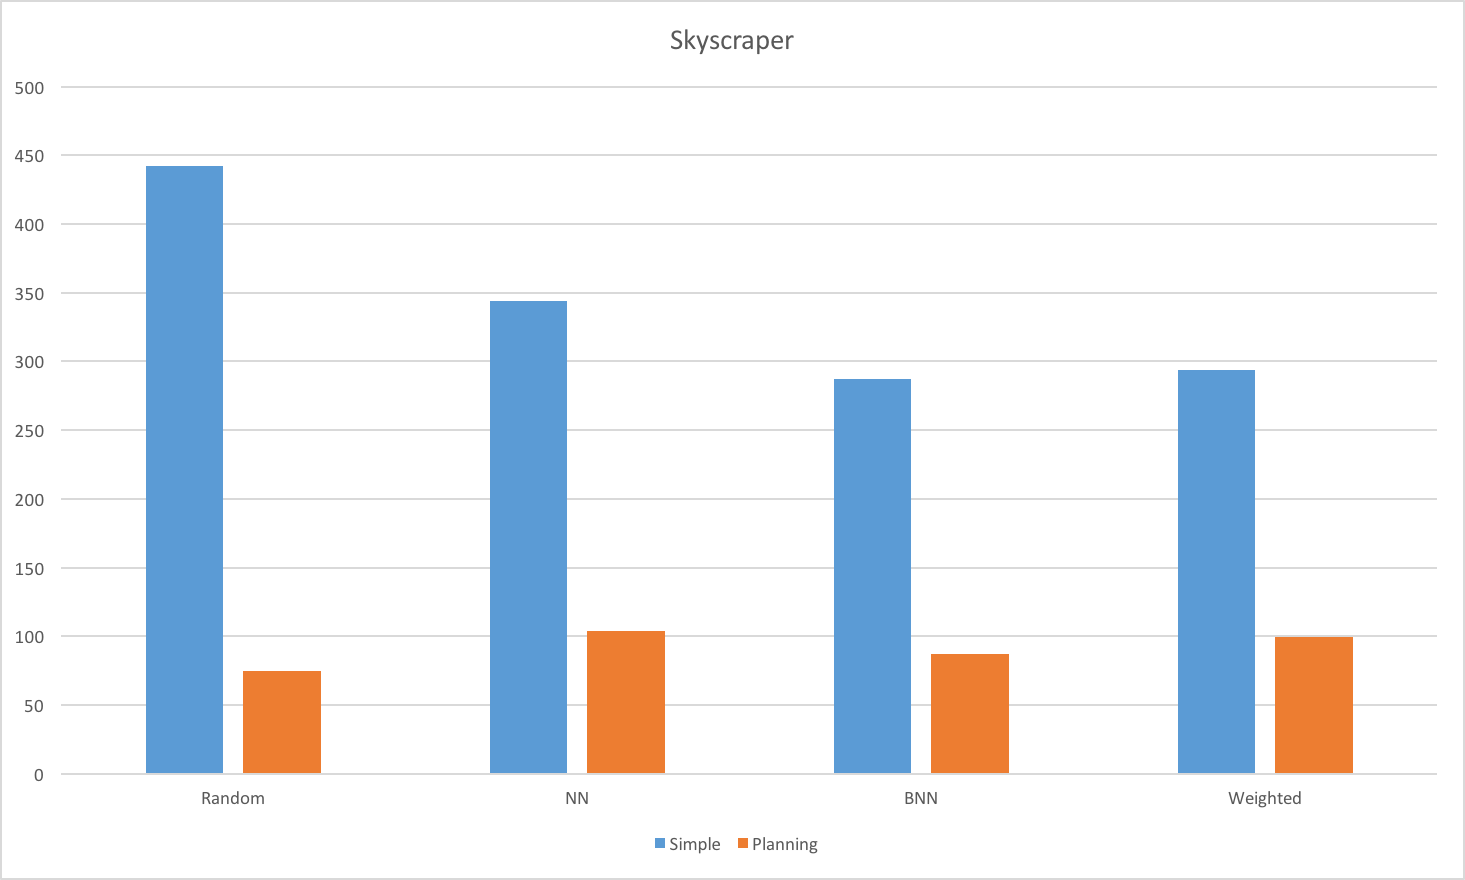
\includegraphics[scale=0.5]{img/chart-averages-skyscraper}
  \caption[{Tempo médio de espera no cenário \textit{Skyscraper}.}]{Tempo médio de espera para diferentes estratégias no cenário \textit{Skyscraper}.}
  \label{fig:result:average:skyscraper}
\end{figure}

\begin{figure}[htb]
  \centering
  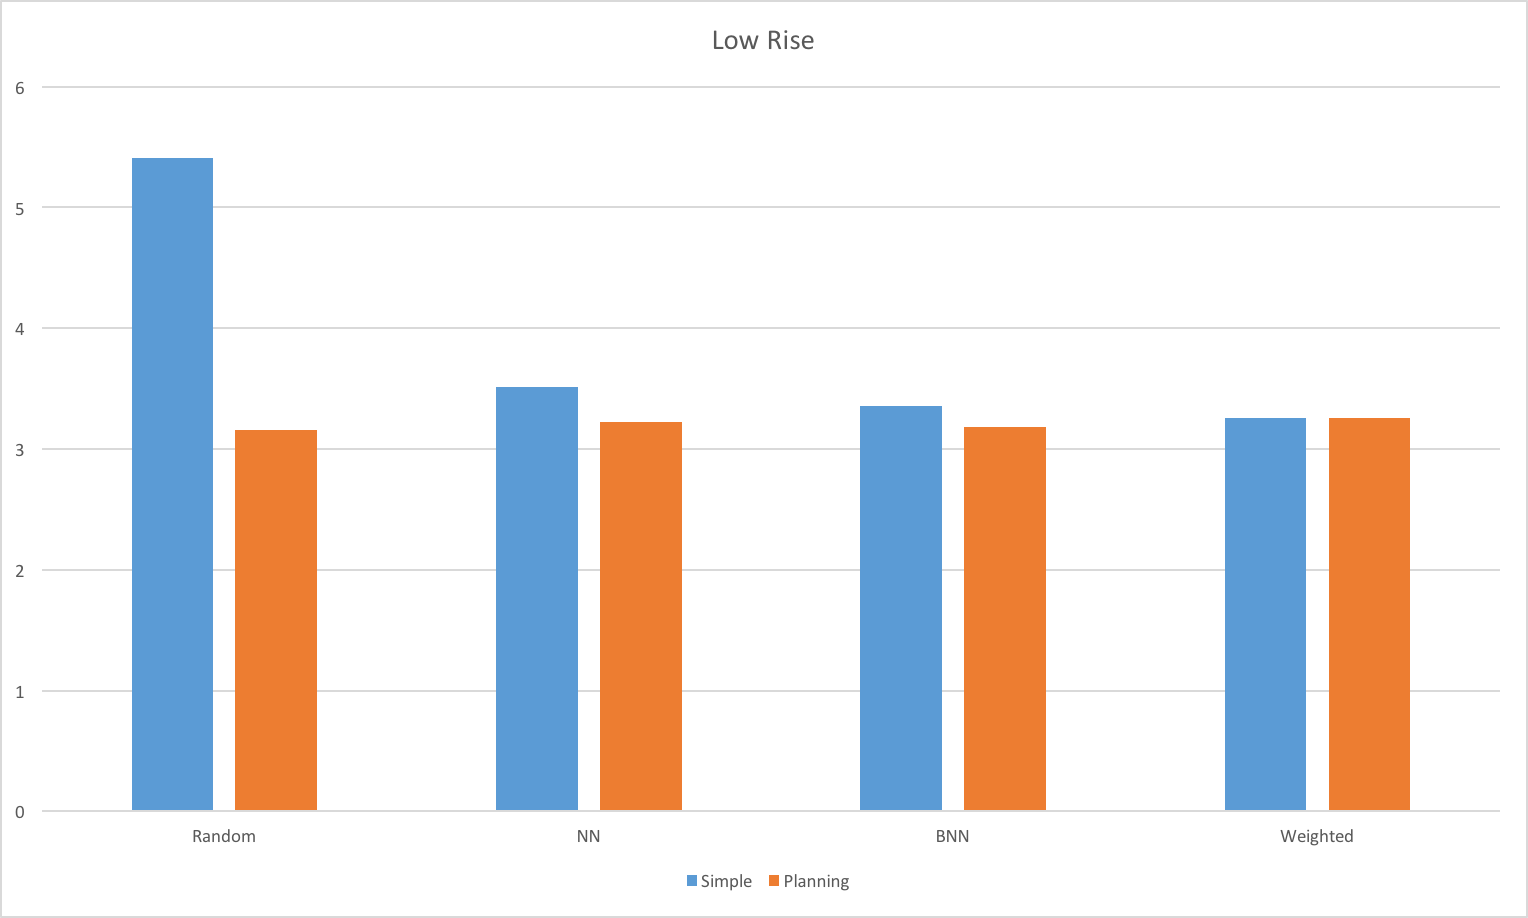
\includegraphics[scale=0.5]{img/chart-averages-low-rise}
  \caption[Tempo médio de espera no cenário \textit{Low-rise}.]{Tempo médio de espera para diferentes estratégias no cenário \textit{Low-rise}.}
  \label{fig:result:average:low-rise}
\end{figure}

\begin{figure}[htb]
  \centering
  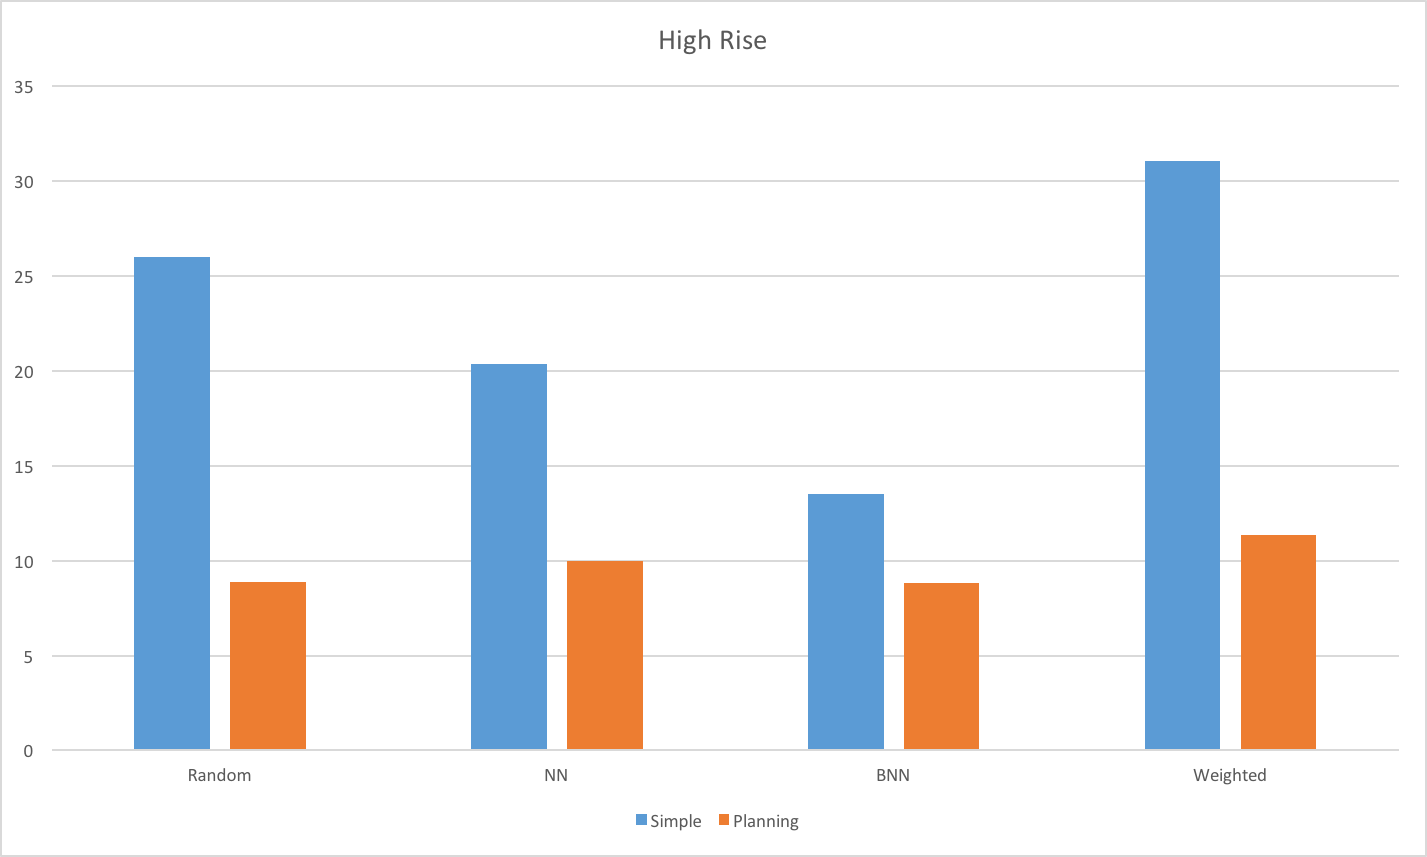
\includegraphics[scale=0.5]{img/chart-averages-high-rise}
  \caption[Tempo médio de espera no cenário \textit{High-rise}.]{Tempo médio de espera para diferentes estratégias no cenário \textit{High-rise}.}
  \label{fig:result:average:high-rise}
\end{figure}